\documentclass{beamer}
\usetheme{CambridgeUS}
\usepackage{amsmath}
\usepackage{amssymb}
\usepackage{tikz}
\usetikzlibrary{arrows.meta, positioning}
\usepackage{cancel}
\usetikzlibrary{positioning}
\usepackage{subcaption}
\usepackage{booktabs}
\usepackage{comment}
\usetikzlibrary{shapes.geometric}
\usepackage{graphicx}



\tikzset{
box/.style={
draw,
rectangle,
rounded corners,
align=left,
font=\small,
inner sep=4pt,
fill=green!15
}
}

\setbeamertemplate{footline}
{
	\leavevmode%
	\hbox{%
		
		% Left: author
		\begin{beamercolorbox}[wd=.2\paperwidth,ht=4ex,dp=1ex,left]{author in head/foot}%
			\hspace{1em}\insertshortauthor
		\end{beamercolorbox}%
		
		% Middle: title
		\begin{beamercolorbox}[wd=.3\paperwidth,ht=4ex,dp=1ex,center]{title in head/foot}%
			\insertshorttitle
		\end{beamercolorbox}%
		
		% Right: logos + slide number
		\begin{beamercolorbox}[wd=.5\paperwidth,ht=4ex,dp=1ex,right]{date in head/foot}%
			
\includegraphics[height=3.5ex]{IFEEL_1.png}\hspace{0.1em}
			
\includegraphics[height=3.5ex]{cofunded_eu.png}\hspace{0.1em}
			
\includegraphics[height=3.5ex]{slo_ministry.png}\hspace{0.1em}
			
\includegraphics[height=3.8ex]{SMASH_CMYK-ENG-horizontal_on_white.pdf}
			\hspace{3.5em}
			\insertframenumber{} / \inserttotalframenumber
			\hspace{1em}
		\end{beamercolorbox}%
	}
}



\title{Neuro-Evolved Heuristics for Variable Gapped Common Subsequence Identification}

\author[Djukanovic et al.  ]{Marko Djukanović\inst{1, 5}  \and
Christian Blum\inst{2}  \and 
Aleksandar Kartelj\inst{3}  \and
Sašo Džeroski\inst{4}  \and
Žiga Zebec\inst{5}
}
 
\institute{ $^1$University of Nova Gorica, Nova Gorica, Slovenia \\ 
$^2$Artificial Intelligence Research Institute (IIIA-CSIC), Barcelona, Spain \\ 
$^3$Faculty of Mathematics, University of Belgrade, Belgrade, Serbia \\
$^4$Jožef Stefan Institute, Ljubljana, Slovenia \ \\
$^5$Institute of Information Sciences (IZUM), Maribor, Slovenia \\ \vspace{0.3cm}

\footnotesize{-- \textcolor{blue}{OPTIMA 2026: XVII International Conference Optimization and Applications, Petrovac, Montenegro} --} \\  \vspace{0.5cm}
\centering

\includegraphics[width=80pt,height=40pt]{IFEEL\_1.png}~\hfill
\includegraphics[width=90pt,height=35pt]{cofunded\_eu.png} ~\hfill
\includegraphics[width=70pt,height=35pt]{slo\_ministry.png}  ~ \hfill

\includegraphics[width=80pt, height=30pt]{SMASH_CMYK-ENG-horizontal_on_white.pdf}
}%slo_ministry.png

\date{}

% Make 


\begin{document}
 
	
\begin{frame}[plain]
    \maketitle
\end{frame}


\begin{frame}{Introduction}
   \begin{itemize}
       \item Objects we deal with: sequences (strings) over finite alphabet  $\Sigma$
       \begin{itemize}
       \item DNA/RNA sequences over $\{\texttt{A}, \texttt{T}, \texttt{G}, \texttt{C/U}\}$
       \item Proteins over 20 (canonical) amino acids: $\{\texttt{A}, \texttt{C}, \texttt{D}, \texttt{E}, \texttt{P}, \texttt{Q} ...\}$ 
       \end{itemize} \vspace{0.3cm}
        \item \textbf{One of central tasks in computational biology:} 
        \begin{itemize}
        	\item  sequence comparison, finding \textbf{common motifs} between sequences
          \item compare structurally, relate it to functionality 
       \end{itemize} \vspace{0.4cm}
       
       \item \textbf{Subsequences}: reveal structural similarities $\rightarrow$ \textcolor{blue}{\textbf{Longest commmon subsequence problem}} variants (studied 50 years already)
   \end{itemize}
\end{frame}

\begin{frame}{Longest common subsequence problem (LCSP)}
   
    
    \begin{definition}[LCSP]
        \textbf{Input}: Given an arbitrary set of sequences $S=\{s_1, \ldots, s_m\}$ \\
        \textbf{Task}: Find a   subsequence $s$  \textcolor{blue}{common} for all sequences from $S$ with \textcolor{blue}{maximum} possible length ($|s|$). 
    \end{definition} \vspace{0.5cm}
    \begin{example}
       Input: $S=$\{\texttt{\textcolor{red}{A}A\textcolor{red}{T}\textcolor{red}{T}G\textcolor{red}{C}}, \texttt{\textcolor{red}{A}\textcolor{red}{T}\textcolor{red}{T}A\textcolor{red}{C}}\} \\ 
       LCS solution: $s=\text{\textcolor{red}{ATTC}}$
    \end{example}
        \vspace{0.3cm}
       % \begin{itemize}
    	%\item Basic problem in computational biology, well-solved  theoretically and practically 
      %\end{itemize}
\end{frame}

\begin{frame}{LCS: Literature \& Problem Variants }
  \begin{itemize}
  \item For $m=2$, polynomially solvable: \textcolor{blue}{Dynamic programming}, Hunt-Szymanski, Hirschenberg,  ... 
 \vspace{0.2cm}
  \item When $m$ arbitrary large -- $\mathcal{NP}$-hard:
   \begin{itemize}
   \item %subject of interest over last 30 years --
    approximation, meta-heuristic, but also exact approaches   
   \end{itemize}  
  \end{itemize}\vspace{0.5cm}
  
  \textbf{Problem-related practical variants}:
  \begin{itemize}
  		\item   Repetition-free, filled LCS problem, \textcolor{red}{Gapped LCS problem}
  \end{itemize}
\end{frame}

\begin{frame}{The gapped LCS problem (Peng and Yang, 2012)}
   \begin{definition}[A gap sequence]
       Given is a sequence $s$ and an assigned function 
       $G_s \colon \{1, \ldots, |s|\} \mapsto \mathbb{N}$. A pair $(s, G_s)$ is called a {gap sequence}.
   \end{definition} (To each position of seq. $s$, one number is assigned) \vspace{0.5cm}
   
   \begin{definition}[A gapped subsequence]
         Sequence $\tilde{s}$ is a \textcolor{red}{gapped subsequence} of $(s, G_s)$ iff 
         \begin{itemize}
             \item $\tilde{s}$ is a \textbf{subsequence} of $s$
             \item the gap constraint $G_s$ fulfilled resp. \textit{positions of embedding} $\tilde{s}$ in $s$:
         \begin{itemize}
             \item  suppose $i_1< \ldots <i_{|\tilde{s}|}$ are those \textbf{positions}  
             \item ($\forall$ $j=2, \ldots, |\tilde{s}|)\, \textcolor{red}{i_{j} - i_{j-1} \leq G_{s}(i_{j})+1}$  (consecutive positions respect gap distances = allowed \textit{number of letters inbetween})
         \end{itemize}
       \end{itemize}
   \end{definition}
   
\end{frame}

\begin{frame}{Problem definition}

   \begin{example}
      $s=\texttt{AATTGC}$, $\textcolor{red}{G_s(\cdot)=1}$
      \begin{itemize}
         \item  $\tilde{s}=\texttt{ATG}$, the embedding: \textcolor{red}{A}A\textcolor{red}{T}T\textcolor{red}{G}C (\textcolor{blue}{valid} gapped subsequence)
         \item  $\tilde{s}=\texttt{ATG}$, the embedding: \textcolor{red}{A}A{T}\textcolor{red}{T}\textcolor{red}{G}C (\textcolor{blue}{invalid} gapped subsequence)
      \end{itemize}
   \end{example} \vspace{0.3cm}
    
   \begin{definition}[The multiple (variable) gapped LCS problem -- MVGLCSP]
        \textbf{Input}: Given is a set of gapped sequences $\{ (s_1, G_{s_1}), \ldots, (s_m, G_{s_m}) \}$. \\
        \textbf{Task}: Find the longest  sequence $\tilde{s}$ so that 
        \begin{itemize}
            \item  $\tilde{s}$ is \textbf{common subusequence} of each $s_i$
            \item $\tilde{s}$ \textbf{fulfills all gap constraints} $G_{s_i}$ ($i=1, \ldots, m$)
        \end{itemize}
    \end{definition}
    \textbf{Note}: When $G_{s_i}=n$ (length of longest sequence) $\Rightarrow$ VGLCSP = LCSP.
\end{frame}

\begin{frame}{Literature \& Motivation for VGLCSP}
   
   \begin{itemize}
       \item  Peng and Yang (2012, 2014): studied  $m=2$  version by \textbf{three dynamic programming} (DP) approaches (basic and two advanced)
       \item  Manea et al. (2024): complexity analysis investigated
       \begin{itemize}
       	\item   \textcolor{red}{NP-hard}  under arbitrary large $m$ 
        \end{itemize} 
        \item Djukanovic et al. (2026): the first approach for general VGLCSP ($m$ arbitrary)
   \end{itemize} \vspace{0.5cm}
   
   \textbf{Motivation}:
   \begin{itemize}
       \item  \textcolor{blue}{Genetics and molecular biology}: DNA/protein comparison analysis where structural distances between residues must be respected \vspace{0.2cm}
       \item \textcolor{blue}{Time-series analysis}: in settings where events are required to occur within specified temporal delays~(Lainscsek et al. (2015))

   \end{itemize}
   
\end{frame}

\begin{frame}{Methodology by Djukanovic et al. (2026) }
	
%	STARTING FROM HERE NEEDS TO BE ADAPTED...
	
    \begin{itemize}
        \item Based on the \textbf{state space graph formulation} of the problem \vspace{0.3cm}
        \item \textbf{Nodes} corresp. to partial solutions and resp. subproblems be solved \vspace{0.3cm}
        \item \textbf{Gap constraints}: incorporated to cut-off invalid extensions (edges) among the LCS extensions immediately \vspace{0.3cm}
        \item \textcolor{red}{\textbf{Many root/source nodes}} in the state graph---the position of leading letter in each common gapped subsequence free to select 
        \begin{itemize}
        	\item   root state space subgraphs (formulation) w.r.t. starting point (match)...
        \end{itemize} 
    \end{itemize}
    
\end{frame}


\begin{comment}
\begin{frame}{Root-based state graph formulation: rough idea}
  
  
  \begin{itemize}
      
      %\item Start with $p^L=1$, and empty partial solution, refers to the complete problem
      
      \item Each \textbf{state} $v=(p^L, l^v)$: one or more feasible partial solutions where
      \begin{itemize}
      	  \item  a vector of positions $p^L$ refer to the positions of suffixes of input sequences relevant to  further expand these sols (subproblem)
      	  \item the  length of current partial solution $l^v$ 
      \end{itemize}\vspace{0.3cm}
      \item \textbf{Expansion} of $v$: extend (concatenate)  partial solutions feasibly (and non-dominantly) by one letter  in all possible ways,  respecting gap constraints \vspace{0.3cm}
      \item \textbf{Non-expandable nodes}: complete solutions; 
  \end{itemize} \vspace{0.15cm}
  
  \fbox{\textcolor{red}{\textbf{Decision: select appropriate (matches)\ $p^L$ for start (empty solution)}}} $\Rightarrow$ possibly \textbf{(exponentially) many root nodes}  \\ \vspace{0.2cm} {Space($p^L$)}: root-based state (sub) graph  induced by root node $(p^L, 0)$.
\end{frame}

\end{comment}

\begin{frame}{Root-based state graph formulation: example}
   
    Given $s_1=$\texttt{\fbox{A}BCA},  $s_2=$\texttt{\fbox{A}CAB}, assuming  $G_1=G_2=1$, match $p^L=(1, 1)$; \\ \vspace{0.3cm} \textsc{SubSpace}($(1, 1)$): partial solutions start with \texttt{A} at $(1, 1)$
   	
   % U nekom delu LaTeX dokumenta:
   \begin{figure}[h!]
   \centering
   \scalebox{0.52}{
   
   
   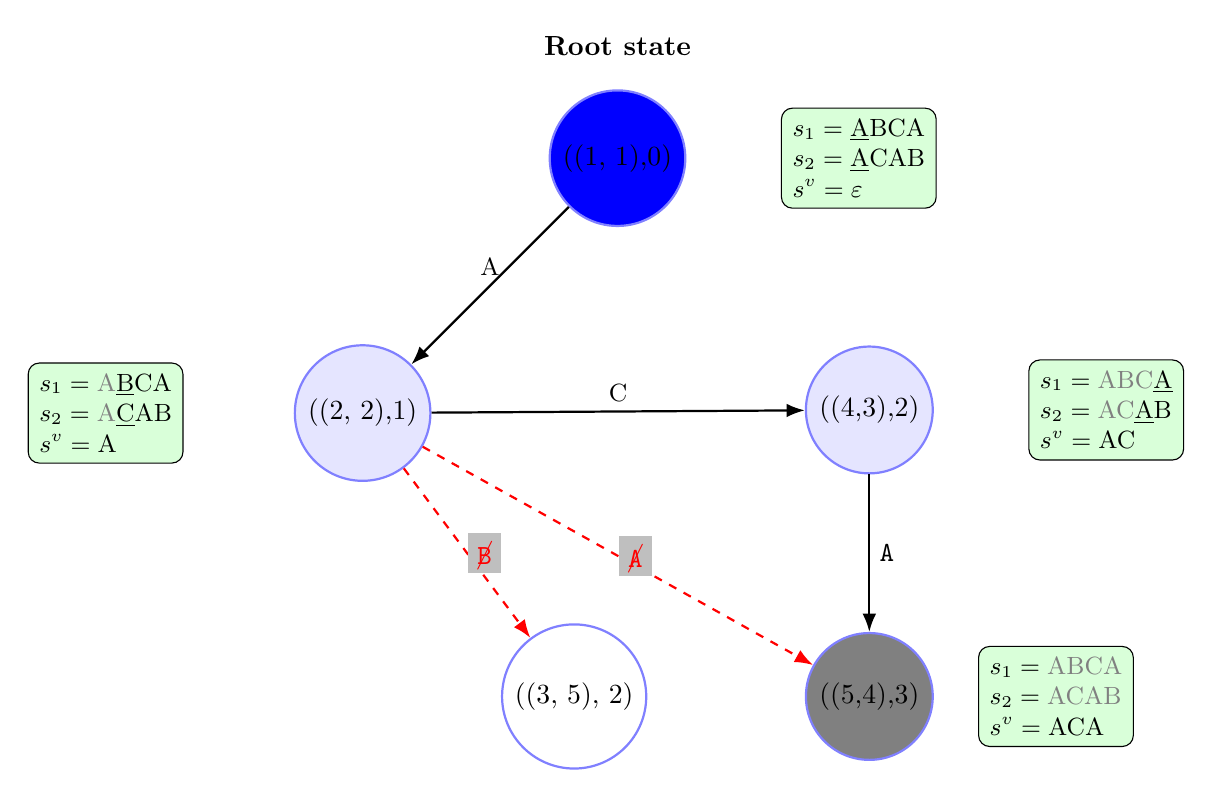
\begin{tikzpicture}[
   state/.style={circle, draw=blue!50, fill=blue!10, thick, minimum size=8mm},
   edge/.style={-Latex, thick},
   node distance=2cm and 2cm
   ]
   
   % Čvorovi
   \node[state, fill=blue] (s0) {((1, 1),0)};
   \node[state, below left=of s0] (s1) {((2, 2),1)};
   \node[state, below right=of s0] (s2) {((4,3),2)};
   %\node[state, below=of s2] (s3) {(4,3)};
   \node[state, below=of s2, fill=gray] (s4) {((5,4),3)}; % krajnje, ali ne koristi se ovde
   \node[state, left=of s4, fill=white] (s5) {((3, 5), 2)}; % krajnje, ali ne koristi se ovde
   
   % Right of root ((1,1),0)
   \node[box, right=12mm of s0] (b0) {
   $s_1=\text{\underline{A}BCA}$\\
   $s_2=\text{\underline{A}CAB}$\\
   $s^v=\varepsilon$
   };
   
   % Left of ((2,2),1)
   \node[box, left=14mm of s1] (b1) {
   $s_1=\text{\textcolor{gray}{A}\underline{B}CA}$\\
   $s_2=\text{\textcolor{gray}{A}\underline{C}AB}$\\
   $s^v=\text{A}$
   };
   
   % Right of ((4,3),2)
   \node[box, right=12mm of s2] (b2) {
   $s_1=\text{\textcolor{gray}{ABC}\underline{A}}$\\
   $s_2=\text{\textcolor{gray}{AC}\underline{A}B}$\\
   $s^v=\text{AC}$
   };
   
   % Right of ((5,4),3)
   \node[box, right=42mm of s5] (b3) {
   $s_1=\text{\textcolor{gray}{ABCA}}$\\
   $s_2=\text{\textcolor{gray}{ACAB}}$\\
   $s^v=\text{ACA}$
   };
   
 
   
   % Grane (samo validne poklapanja)
   \draw[edge] (s0) -- node[above] {\small A} (s1);
   %\draw[edge] (s0) -- node[above] {\small A} (s2);
   \draw[edge] (s1) -- node[above] {\small C} (s2);
   %\draw[edge] (s2) -- node[right] {\small A} (s3);
   %\draw[edge] (s3) -- node[right] {\texttt{A}} (s4);
   \draw[edge,  scale=2.2, dashed, red] (s1) -- node[right, fill=lightgray] {$\cancel{\texttt{B}}$} (s5);
   
    \draw[edge,  scale=2.2, dashed, red] (s1) -- node[right, fill=lightgray] {$\cancel{\texttt{A}}$} (s4);
   % Oznake
   \node[above=0.3cm of s0] {\textbf{Root state}};
   %\node[below=1.5cm of s3] {\small \textbf{Krajnje stanje}};
   \draw[edge] (s2) -- node[right] {\texttt{A}} (s4);
   
   \end{tikzpicture}}
   
   %\caption{State space graph Space($r=((1, 1), 0)$) for MVGLCSP between the sequences \texttt{\fbox{A}BCA} and  \texttt{\fbox{A}CAB}, assuming $\textcolor{red}{G_1=G_2=1}$.   % \fxnote{Add VGLCS example}
   %}
   
   \label{fig:vgcs-grafstanja}
   \end{figure}
   $\textcolor{red}{\textsc{SubSpace}((1, 1)) \Longrightarrow \texttt{ACA}}$
   \end{frame}



\begin{frame}{An issue with the root-state-space formulation: disconnected components}
	
	\begin{example}
		$
		S = \{ s_1 = \texttt{ATGG\fbox{A}AA},\; s_2 = \texttt{ATCC\fbox{A}AA} \},
		$
		with $G_{s_1} = G_{s_2} = 1$. 
	\end{example}
	
	\centering
	\scalebox{0.33}{
		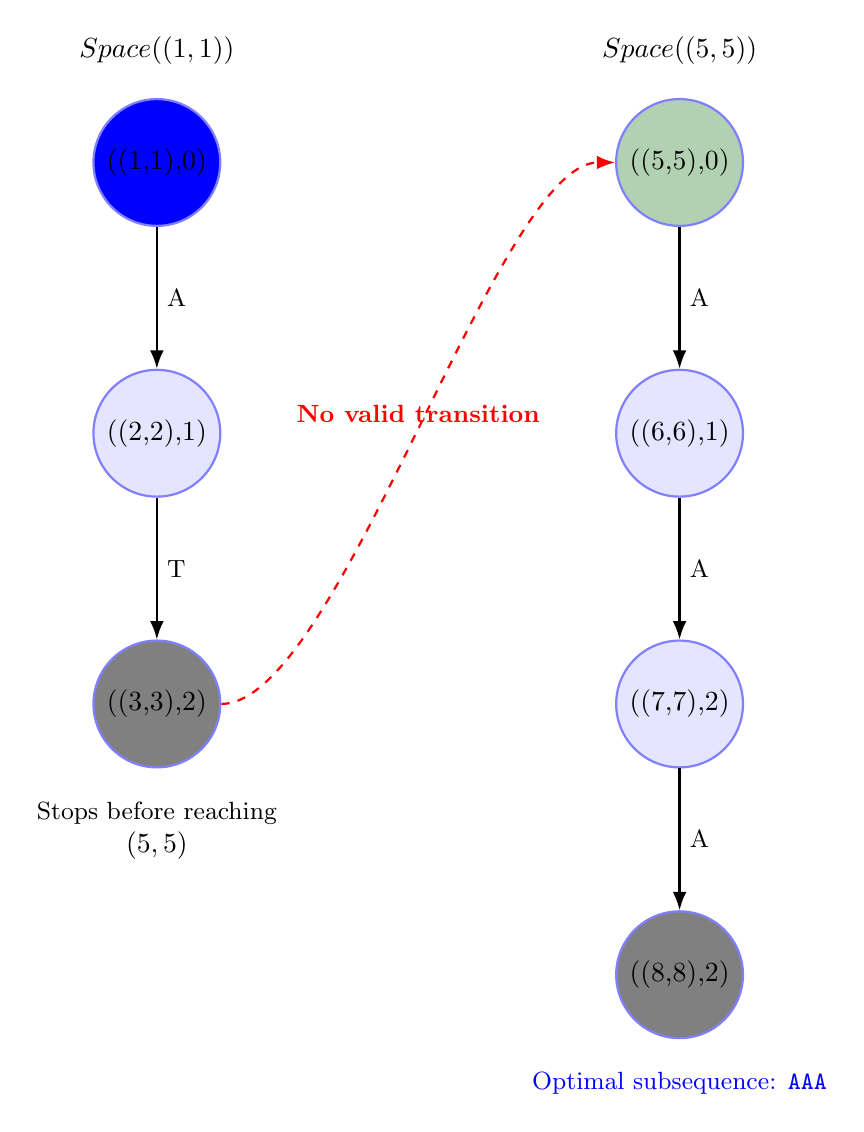
\begin{tikzpicture}[
			state/.style={circle, draw=blue!50, fill=blue!10, thick, minimum size=8mm},
			edge/.style={-Latex, thick},
			invalid/.style={-Latex, thick, dashed, red},
			node distance=1.8cm
			]
			
			% ---------------- LEFT COMPONENT ----------------
			\node[state, fill=blue] (r1) at (0,0) {((1,1),0)};
			\node[state, below=of r1] (a1) {((2,2),1)};
			\node[state, below=of a1, fill=gray] (a2) {((3,3),2)};
			
			\draw[edge] (r1) -- node[right] {\small A} (a1);
			\draw[edge] (a1) -- node[right] {\small T} (a2);
			
			\node[above=0.3cm of r1] {\textbf{$Space((1,1))$}};
			\node[below=0.3cm of a2, align=center] {\small Stops before reaching \\ $(5,5)$};
			
			% ---------------- RIGHT COMPONENT ----------------
			\node[state, fill=green!40!black!30, right=5cm of r1] (r2) {((5,5),0)};
			\node[state, below=of r2] (b1) {((6,6),1)};
			\node[state, below=of b1] (b2) {((7,7),2)};
			\node[state, below=of b2, fill=gray] (b3) {((8,8),2)};		
			\draw[edge] (r2) -- node[right] {\small A} (b1);
			\draw[edge] (b1) -- node[right] {\small A} (b2);
			\draw[edge] (b2) -- node[right] {\small A} (b3);
						
			\node[above=0.3cm of r2] {\textbf{$Space((5,5))$}};
			\node[below=0.3cm of b3] {\small \textcolor{blue}{Optimal subsequence: \texttt{AAA}}};
			
			% ---------------- DISCONNECTION INDICATOR ----------------
			\draw[invalid] (a2.east) .. controls +(1.5,0) and +(-1.5,0) .. 
			node[above] {\small \textbf{No valid transition}} (r2.west);
			
		\end{tikzpicture}
	}
	
	
	\footnotesize{\textbf{Observation:}$
	((5,5),\ast) \notin \textsc{SubSpace}((1,1))	$, \textcolor{red}{The optimal solution: \texttt{AAA}.}}
	
	%\vspace{0.1cm}
	
	%\textcolor{blue}{\textbf{Fix:}} Use a multi-root formulation (e.g., multi-source beam search).
	
\end{frame}


\begin{comment}
\begin{frame}{Iterative multi-source beam search (IMSBS) strategy}
      
      \begin{itemize}
      	%	\item \textbf{Full state space} of a VGLCSP instance: $\bigcup_{v \in \mathcal{R}} \mathrm{Space}(\mathbf{p}^{L, v})$, with $v=(\mathbf{p}^{L, v}, 0) \in \mathcal{R}$ all root states  
      		\item Explicitly enumerating root states computationally prohibitive ($O(n^m)$ time) \vspace{0.7cm}
      		\item \textcolor{red}{\textbf{IMSBS}} (rough idea of exploring space of root nodes):  \vspace{0.2cm}
      		\begin{enumerate}
      		    \item  \textbf{Exploitation} of  \text{Space}($p^L$): given to \textcolor{blue}{beam search} (BS) --- limited breadth-first-search (BFS) strategy;  {parameter $\beta$} controls the number of nodes at each level to further pursue \vspace{0.5cm}
      		    
      		    \item \textbf{Exploration} of promising regions (\text{Space}($p^L$)) of the state space  
      		    \begin{itemize}
      		       \item  \textbf{Iteratively identify} a set of \textcolor{red}{promising} candidate root states during BS
      		       \item allow some (non-) root nodes: effective \textit{refinement} (find \textcolor{red}{distant root ancestors} to reach that node)
      		    \end{itemize}
      		\end{enumerate}
      \end{itemize}  
\end{frame}

\end{comment}


\begin{comment}
\begin{frame}{Components and characteristics of IMSBS}
     TODO: Consider not to display this slide!
     
   \begin{itemize}
     	\item $\mathcal{R}$: a \textbf{global set} of root-node candidates, dynamically updated over iterations
     	\item \textbf{Beam search} (\textbf{backward}): not all candidate nodes from $\mathcal{R}$ are root nodes
     	\begin{itemize}
     		\item \textcolor{blue}{\textbf{refine}} them by performing the  {backward} approximate (BS) passes from candidate root nodes to effectively reach distant (real) \textcolor{red}{root node} in the state space
     	\end{itemize}
     	\item  {\textbf{Beam search}} (\textbf{forward}): \textcolor{red}{intensification} in the current root (sub-)space {Space($p$)} -- seek for high-quality (complete) solutions in the corresponding search sub-regions
     	\item \textcolor{red}{diversification}:  during each BS (forward), complete nodes expanded in all possible ways (\textbf{gaps ignored}) to generate candidates for roots (distant from the current region)
     \end{itemize}

\end{frame}
\end{comment}

\begin{frame}{Workflow of the Iterative Multi-source Beam Search -- IMSBS}
 
	 %\begin{figure}[!ht]
	 \centering
	 \scalebox{0.40}{
	 	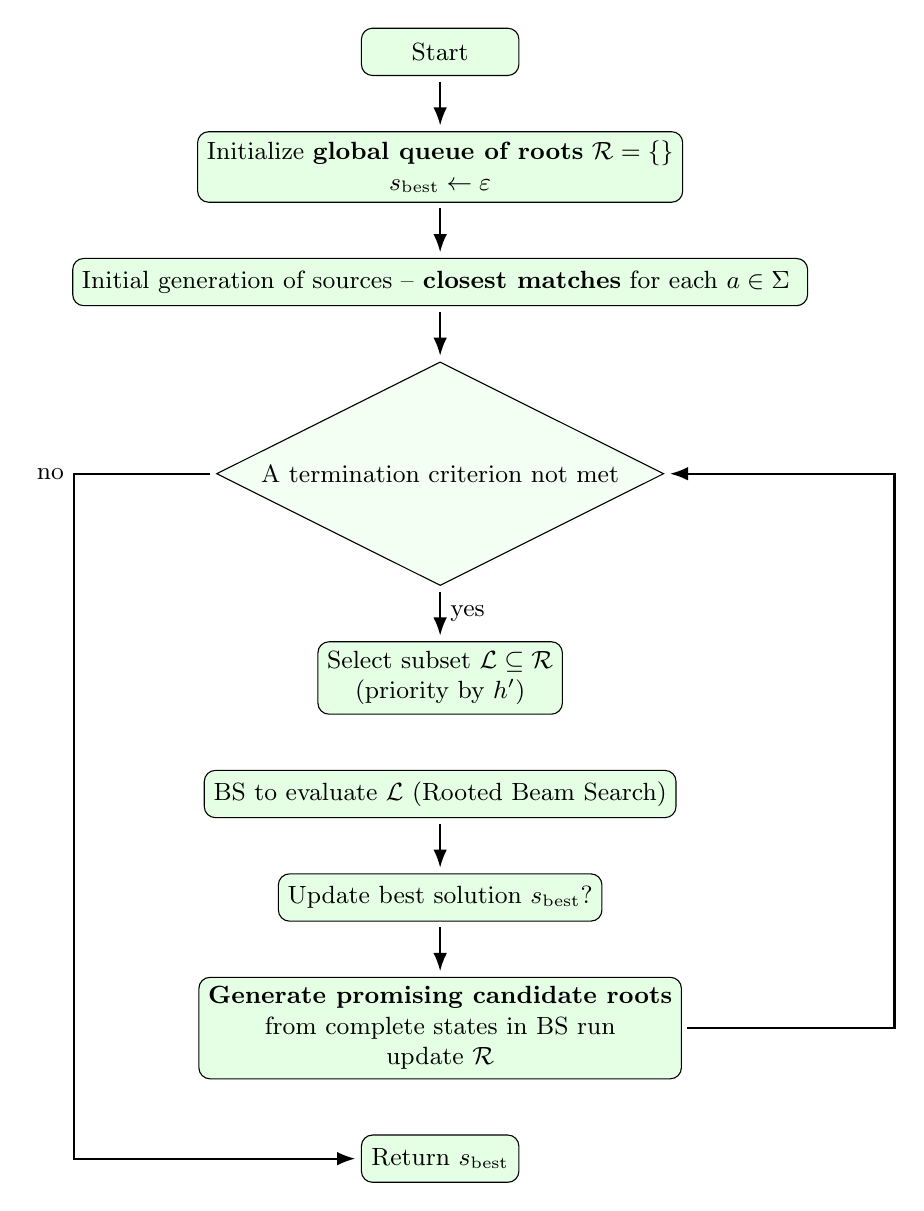
\begin{tikzpicture}[
	 		node distance=0.7cm and 1.2cm,
	 		every node/.style={font=\small},
	 		block/.style={
	 			rectangle,
	 			draw,
	 			rounded corners,
	 			align=center,
	 			minimum width=2.0cm,
	 			minimum height=0.6cm,
	 			fill=green!10
	 		},
	 		decision/.style={
	 			diamond,
	 			draw,
	 			align=center,
	 			aspect=2,
	 			fill=green!5
	 		},
	 		arrow/.style={
	 			->,
	 			thick,
	 			>=Latex,
	 			shorten >=2pt,
	 			shorten <=2pt
	 		}
	 		]
	 		
	 		% Nodes
	 		\node[block] (start) {Start};
	 		
	 		\node[block, below=of start] (init) {Initialize \textbf{global queue of roots} $\mathcal{R}=\{\}$\\
	 			$s_{\text{best}} \leftarrow \varepsilon$};
	 		
	 		\node[block, below=of init] (expandR) {Initial generation of sources -- \textbf{closest matches} for each $a \in \Sigma$ };
	 		
	 		\node[decision, below=of expandR] (while) {A termination criterion not met};
	 		
	 		\node[block, below=of while] (selectL) {Select subset $\mathcal{L} \subseteq \mathcal{R}$\\
	 			(priority by $h'$)};
	 		
	 		%\node[block, below=of selectL] (backward) {\textbf{Refinement} of $v \in \mathcal{L}$ \\ (Rooted BS on reversed prefixes w.r.t.\ $p^{L,v}$)};
	 		
	 		\node[block, below=of selectL] (forward) {BS to evaluate $\mathcal{L}$ 
	 			(Rooted Beam Search)};
	 		
	 		\node[block, below=of forward] (updateBest) {Update best solution $s_{\text{best}}?$};
	 		
	 		\node[block, below=of updateBest] (expandNew) {\textbf{Generate promising  candidate roots} \\ from complete states in BS run \\ update $\mathcal{R}$};
	 		
	 		\node[block, below=of expandNew] (end) {Return $s_{\text{best}}$};
	 		
	 		% Arrows (main flow)
	 		\draw[arrow] (start) -- (init);
	 		\draw[arrow] (init) -- (expandR);
	 		\draw[arrow] (expandR) -- (while);
	 		
	 		\draw[arrow] (while) -- node[right] {yes} (selectL);
	 		%\draw[arrow] (selectL) -- (backward);
	 		%\draw[arrow] (backward) -- (forward);
	 		\draw[arrow] (forward) -- (updateBest);
	 		\draw[arrow] (updateBest) -- (expandNew);
	 		
	 		% Explicit loop-back arrow (FIXED)
	 		 \draw[arrow]
	 		(expandNew.east) -- ++(2.7,0)
	 		|- (while.east);
	 		
	 		% Exit arrow
	 		\draw[arrow]
	 		(while.west) -- ++(-1.8,0)
	 		node[left] {no}
	 		|- (end.west);
	 		
	 	\end{tikzpicture}
	 }
	 
	 	%\caption{Simplified workflow of the Iterated Multi-source Beam Search (IMSBS) framework.}
	 	%\label{fig:imsbs_workflow}
	 %\end{figure}
	 	 		
	 %\node[block, below=of expandNew] (iter) {$iter \leftarrow iter + 1$};
	 	 		%\draw[arrow] (expandNew) -- (iter);
 
\end{frame}

%\begin{frame}{The core advantages of the IMSBS}
% 
%     \begin{itemize}
%     	\item Balance between complete beam search execution (local exploration of promising paths) and the generation of new, promising source nodes (\textcolor{red}{\textbf{global coverage}} of generally weakly-connected search space) \vspace{0.3cm}
%     	\item Preventing from direct suboptimal solutions reduced by employing backward beam search procedure (\textcolor{red}{\textbf{refinement}})
%     \end{itemize}
%      
%\end{frame}

\begin{frame}{Heuristic guidances in IMSBS}
    
    Three LCS heuristic guidances to guide BS and prioritize root nodes most sensible: \vspace{0.2cm}
        \begin{enumerate}
    	  	\item   $\textrm{UB}_2$: \textit{Character Frequency Alignment} score the best performing
    \end{enumerate}
    
    Experimental evaluation -- Conclusions:
    \begin{itemize}
    	\item IMSBS able to efficiently run on large synthetic instances
    	\item Obtain a large portion  of known optimal solutions for $m=2$
    	\item \textbf{Weaknesses}: the performance of $\textrm{UB}_2$ seems to significantly drop for  large $n$ ($n=500$) and small $|\Sigma|$ ($|\Sigma|=2$)
    \end{itemize} \vspace{0.7cm}
    $\Rightarrow$ \textcolor{red}{\textbf{Construction of a new heuristic guidance}}
\end{frame}


\begin{frame}{Designing advanced heuristic guidances }
TODO
\end{frame}

 
\end{document}
